%%%%%%%%%%%%%%%%%%%%%%%%%%%%%%%%%%%%%%%%%%%%%%%%%%%%%%%%%%%%%%%%%%%%%%%%%%%%%%%%%%%%
% Document data
%%%%%%%%%%%%%%%%%%%%%%%%%%%%%%%%%%%%%%%%%%%%%%%%%%%%%%%%%%%%%%%%%%%%%%%%%%%%%%%%%%%%
\documentclass[12pt]{article} %report allows for chapters
%%%%%%%%%%%%%%%%%%%%%%%%%%%%%%%%%%%%%%%%%%%%%%%%%%%%%%%%%%%%%%%%%%%%%%%%%%%%%%%%%%%%
\usepackage{preamble}
\newcommand{\grad}{\boldsymbol{\vec{\nabla}}}
\newcommand{\curvegamma}{\boldsymbol{\vec{\gamma}}}
\newcommand{\tangentgamma}{\boldsymbol{\dot{\vec{\gamma}}}}
\newcommand{\vecfieldE}{\boldsymbol{\vec{E}}}
\newcommand{\rhat}{\boldsymbol{\hat{r}}}
\newcommand{\thetahat}{\boldsymbol{\hat{\theta}}}
\newcommand{\phihat}{\boldsymbol{\hat{\phi}}}
\newcommand{\unitvec}{\boldsymbol{\hat{n}}}
\begin{document}

\begin{center}
   \textsc{\large MATH 272, Homework 8, \emph{Solutions}}\\
   \textsc{Due April 6$^\textrm{th}$}
\end{center}
\vspace{.5cm}

\begin{problem}
    Plot each of the following vector fields.
    \begin{enumerate}[(a)]
        \item $\rhat = \frac{x}{\sqrt{x^2+y^2+z^2}}\xhat + \frac{y}{\sqrt{x^2+y^2+z^2}}\yhat+\frac{z}{\sqrt{x^2+y^2+z^2}}\zhat$.
        \item $\thetahat = \frac{-y}{\sqrt{x^2+y^2}}\xhat + \frac{x}{\sqrt{x^2+y^2}}\yhat$.
        \item $\phihat = \frac{xz}{\sqrt{x^2+y^2}\sqrt{x^2+y^2+z^2}}\xhat + \frac{yz}{\sqrt{x^2+y^2}\sqrt{x^2+y^2+z^2}}\yhat+\frac{-\sqrt{x^2+y^2}}{\sqrt{x^2+y^2+z^2}}\zhat$.
    \end{enumerate}
\end{problem}
\begin{solution}
~
\begin{enumerate}[(a)]
    \item Here is the plot for $\rhat$.
    \begin{figure}[H]
        \centering
        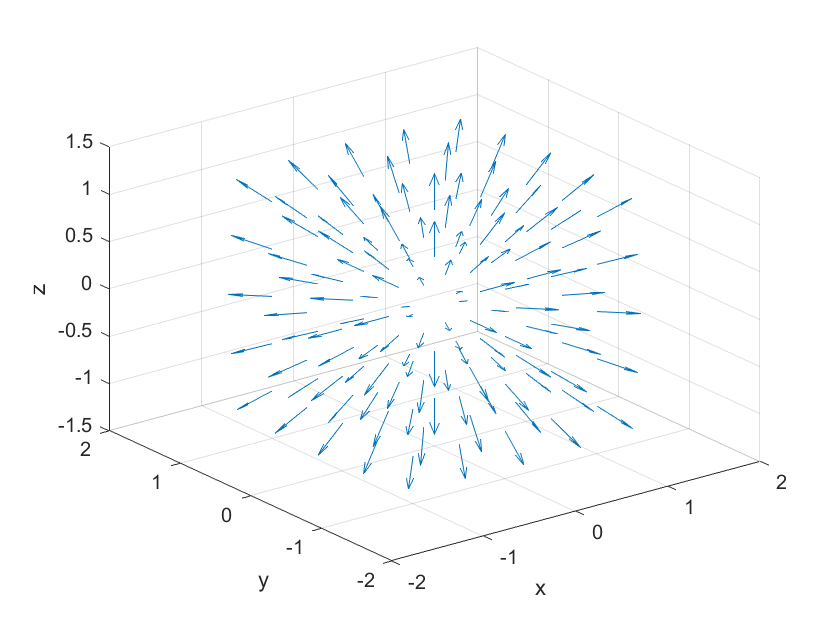
\includegraphics[width=.8\textwidth]{r_hat.png}
    \end{figure}
        \item Here is the plot for $\thetahat$.
        \begin{figure}[H]
            \centering
            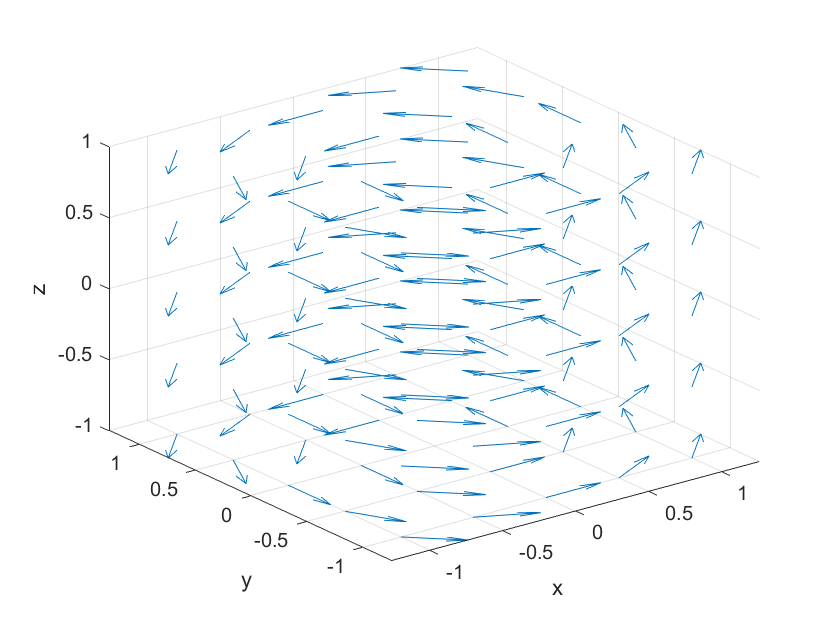
\includegraphics[width=.8\textwidth]{theta_hat.png}
        \end{figure}
    \item Here is the plot for $\phihat$.
    \begin{figure}[H]
        \centering
        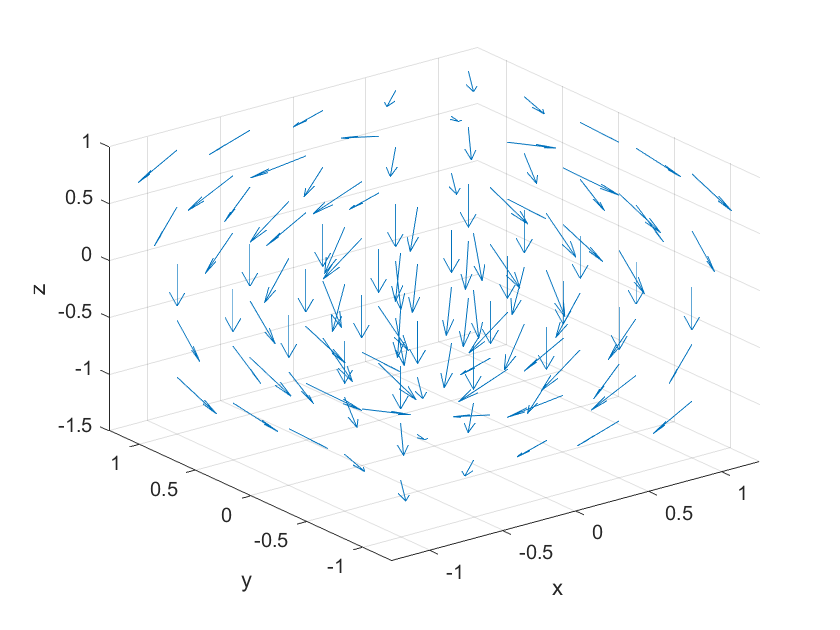
\includegraphics[width=.8\textwidth]{phi_hat.png}
    \end{figure}        
\end{enumerate}
\end{solution}

\newpage
\begin{problem}
    Consider the following vector field
    \[
    \vecfieldE = \frac{x}{\left(x^2+y^2+z^2\right)^{3/2}} \xhat + \frac{y}{\left(x^2+y^2+z^2\right)^{3/2}} \yhat + \frac{z}{\left(x^2+y^2+z^2\right)^{3/2}} \zhat,
    \]
    which you can think of as the electric field of a positive point charge.  We argued that this field $\vecfieldE$ is conservative in a previous homework problem. Specifically, $\vecfieldE = \grad \phi$, for some scalar field $\phi$. This follows from Faraday's law for static charges.
    \begin{enumerate}[(a)]
        \item Compute the integral
        \[
        T=\int_{\curvegamma} \vecfieldE \cdot d\curvegamma \qquad \textrm{where} \qquad \curvegamma(t) = \begin{pmatrix} t \\ t \\ t \end{pmatrix},
        \]
        and $a\leq t \leq b$ with $a$ and $b$ both greater than 0.  Note that this integral $T$ describes the gain in kinetic energy of a charged particle that moved along the path $\curvegamma$. 
        \item Equivalently, since $\vecfieldE$ is conservative, we have
        \[
        T=\int_{\curvegamma} \vecfieldE \cdot d\curvegamma = \phi(\curvegamma(b))-\phi(\curvegamma(a)).
        \]
        Show that this is true for the given vector field and potential. This shows that the choice of path does not matter; only the endpoints $\curvegamma(a)$ and $\curvegamma(b)$ matter.
        \item Argue why the integral around any closed curve must be zero.
    \end{enumerate}
\end{problem}
\begin{solution}
\begin{enumerate}[(a)]
    \item First, note that
    \[
    d\curvegamma = \tangentgamma dt = (\xhat + \yhat + \zhat)dt.
    \]
    Thus, we have that
    \[
    \vecfieldE \cdot d\curvegamma = \frac{x+y+z}{\left(x^2+y^2+z^2\right)^{3/2}}dt.
    \]
    Now, we have
    \begin{align*}
        \int_{\curvegamma} \vecfieldE \cdot d\gamma &= \int_a^b \frac{t+t+t}{\left(t^2+t^2+t^2\right)^{3/2}} dt\\
        &= \int_a^b \frac{3t}{(3t^2)^{3/2}}dt\\
        &= \int_a^b \frac{1}{\sqrt{3}} \frac{1}{t^2} dt\\
        &= \frac{-1}{\sqrt{3}}\left(\frac{1}{b} - \frac{1}{a}\right).
    \end{align*}
    \item Note that we have
    \[
    \phi(x,y,z) = \frac{-1}{\sqrt{x^2+y^2+z^2}},
    \]
    from previous homeworks.  Then, we have
    \begin{align*}
        \phi(\curvegamma(b))-\phi(\curvegamma(a)) &= \frac{-1}{\sqrt{b^2+b^2+b^2}}-\frac{1}{\sqrt{a^2+a^2+a^2}}\\
        &= \frac{-1}{\sqrt{3}} \left(\frac{1}{b}-\frac{1}{a}\right)
    \end{align*}
    \item For a closed curve, we have $\curvegamma(b)=\curvegamma(a)$ and thus
    \[
    \int_{\curvegamma} \vecfieldE \cdot d\gamma = \phi(\curvegamma(b))-\phi(\curvegamma(a)) = \phi(\curvegamma(a))-\phi(\curvegamma(a))=0.
    \]
\end{enumerate}
\end{solution}

\newpage
\begin{problem}
    Let us see some of the benefit of using spherical coordinates. 
    \begin{enumerate}[(a)]
        \item Using the fact that 
        \[
        \rhat = \frac{x}{\sqrt{x^2+y^2+z^2}}\xhat + \frac{y}{\sqrt{x^2+y^2+z^2}}\yhat + \frac{z}{\sqrt{x^2+y^2+z^2}}\zhat,
        \]
        convert the vector field $\vecfieldE$ into spherical coordinates (i.e., only a function of $r$, $\theta$, $\phi$, and $\rhat$, $\thetahat$, and $\phihat$).
        \item Parameterize the surface of a sphere of radius $R$ (which we'll call $\Sigma$) as well as the outward normal vector $\unitvec$ and  in spherical coordinates.
        \item Compute the following integral using spherical coordinates that we have found:
        \[
        \iint_\Sigma \vecfieldE \cdot \unitvec d\Sigma,
        \]
        where $d\Sigma$ will be the area form in spherical coordinates.
    \end{enumerate}
\end{problem}
\begin{solution}~
\begin{enumerate}[(a)]
    \item We have
    \begin{align*}
    \vecfieldE &= \frac{x}{\left(x^2+y^2+z^2\right)^{3/2}} \xhat + \frac{y}{\left(x^2+y^2+z^2\right)^{3/2}} \yhat + \frac{z}{\left(x^2+y^2+z^2\right)^{3/2}} \zhat\\
     &= \frac{1}{x^2+y^2+z^2} \left( \frac{x}{\sqrt{x^2+y^2+z^2}} \xhat + \frac{y}{\sqrt{x^2+y^2+z^2}} \yhat + \frac{z}{\sqrt{x^2+y^2+z^2}} \zhat\right)\\
     &= \frac{1}{x^2+y^2+z^2} \rhat\\
     &= \frac{1}{r^2} \rhat.
    \end{align*}
    \item We have the parameterization of the surface of a unit sphere given by letting $r=R$ and $\theta \in [0,2\pi)$ and $\phi \in [0,\pi]$.  If we then attempt to compute the unit vector, we can use the implicit equation 
    \[
    f(x,y,z)=x^2+y^2+z^2=R^2.
    \]
    From this, we have
    \begin{align*}
        \unitvec &= \frac{\grad f}{\left| \grad f \right|} \\
        &= \frac{2x}{\sqrt{4x^2+4y^2+4z^2}}\xhat + \frac{2y}{\sqrt{4x^2+4y^2+4z^2}}\yhat + \frac{2z}{\sqrt{4x^2+4y^2+4z^2}}\zhat\\
        &= \rhat.
    \end{align*}
    \item From the previous work, we have that
    \[
    \vecfieldE \cdot \unitvec = \frac{1}{r^2}.  
    \]
    Then, this gives us
    \begin{align*}
        \iint_{\Sigma} \vecfieldE \cdot \unitvec d\Sigma &= \int_0^\pi \int_0^{2\pi} \frac{1}{R^2} R^2 \sin \phi  \, d\theta \, d\phi \\
        &= 2\pi \int_0^\pi \sin \phi \, d \phi\\
        &= 4 \pi.  
    \end{align*}
    One can notice that the radius of the sphere does not come into play here.
\end{enumerate} 
\end{solution}

\newpage
\begin{problem}
    Note that the Laplacian $\Delta$ in cylindrical coordinates is given by
    \[
        \Delta f(\rho,\theta,z) = \frac{1}{\rho} \frac{\partial}{\partial \rho} \left(\rho \frac{\partial f}{\partial \rho}\right)+\frac{1}{\rho^2}\frac{\partial^2 f}{\partial \theta^2} + \frac{\partial^2 f}{\partial z^2}.
    \]
    Compute the Laplacian of
    \[
        f(\rho,\theta,z) = \sqrt{\rho^2+z^2} z \cos(\theta).
    \]
\end{problem}
\begin{solution}
Let's compute each term and then add them together. We have
\begin{align*}
    A=\frac{1}{\rho}\frac{\partial}{\partial \rho} \left(\rho \frac{\partial f}{\partial \rho} \right) &=  \frac{z\cos \theta}{\rho} \frac{\partial}{\partial \rho} \left( \frac{\rho^2}{\sqrt{\rho^2+z^2}} \right)\\
    &=\frac{z\cos \theta}{\rho} \left(\frac{2\rho}{\sqrt{\rho^2+z^2}}-\frac{\rho}{\left(\rho^2+z^2\right)}\right)\\
    &= z\cos \theta \left( \frac{2}{\sqrt{\rho^2+z^2}} - \frac{1}{\left(\rho^2+z^2\right)}\right).
\end{align*}
Likewise, we have
\begin{align*}
    B=\frac{1}{\rho^2} \frac{\partial^2 f}{\partial \theta^2} &= -\frac{\sqrt{\rho^2+z^2}z\cos\theta}{\rho^2}.
\end{align*}  
Lastly, we have
\begin{align*}
    C=\frac{\partial^2 f}{\partial z^2} &= \cos \theta \frac{\partial}{\partial z}\frac{\partial}{\partial z} \left( z \sqrt{\rho^2+z^2}\right)\\
    &= \cos \theta \frac{\partial}{\partial z} \left( \sqrt{\rho^2+z^2}+ \frac{z^2}{\sqrt{\rho^2+z^2}}\right)\\
    &= \cos \theta \left(\frac{z}{\sqrt{\rho^2+z^2}}+\frac{2z}{\sqrt{\rho^2+z^2}}-\frac{z^3}{\left(\rho^2+z^2\right)^{3/2}}\right).
\end{align*}
Then we have that
\[
\Delta f = A+B+C.
\]
\end{solution}

\newpage
\begin{problem}
    Note that the Laplacian $\Delta$ in spherical coordinates is given by
    \[
        \Delta f(r,\theta,\phi) = \frac{1}{r^2} \frac{\partial}{\partial r} \left(r^2 \frac{\partial f}{\partial r}\right)+\frac{1}{r^2 \sin(\theta)}\frac{\partial}{\partial \theta} \left(\sin(\theta) \frac{\partial f}{\partial \theta}\right) + \frac{1}{r^2 \sin^2 (\theta)} \frac{\partial^2 f}{\partial \phi^2}.
    \]
    Compute the Laplacian of
    \[
       f(r,\theta,\phi) = r^2 \cos(\theta)\cos(\phi).
    \]
\end{problem}
\begin{solution}
 Again, we will do this piece by piece. First, we have
 \begin{align*}
    A=\frac{1}{r^2}\frac{\partial}{\partial r} \left(r^2 \frac{\partial f}{\partial r}\right)&= \frac{\cos \theta \cos \phi}{r^2}\frac{\partial}{\partial r} \left(2r^3\right) \\
    &= \frac{\cos \theta \cos\phi}{r^2} 6r^2\\
    &= 6 \cos \theta \cos \phi.
 \end{align*}
 Next, we have
 \begin{align*}
    B=\frac{1}{r^2 \sin \theta} \frac{\partial}{\partial \theta} \left(\sin \theta \frac{\partial f}{\partial \theta}\right) &= \frac{\cos \phi}{\sin \theta} \frac{\partial}{\partial \theta} \left( -\sin^2 \theta\right)\\
    &=-2\cos \theta \cos \phi.
 \end{align*}
 Lastly, we have
 \begin{align*}
    C=\frac{1}{r^2\sin^2 \theta} \frac{\partial^2 f}{\partial \phi^2}&= \frac{\cos \theta}{\sin^2 \theta} \left(-\cos \phi\right)\\
    &= \frac{-\cos \theta \cos \phi}{\sin^2 \theta}.
 \end{align*}
 Then,
 \[
 \Delta f = A+B+C.
 \]
\end{solution}

\newpage
\begin{problem} (BONUS)
The following problem is a somewhat pop-culture math paradox known as the \emph{napkin ring problem} (see Vsauce for more).  Consider the following problem.  We want to compute the volume inside a ball of radius $R$ after drilling out an inscribed cylinder of height $h$. See the following picture.
\begin{figure}[H]
	\centering
	\def\svgwidth{0.60\columnwidth}
	\input{Sphere_Bands.pdf_tex}
\end{figure}
The question is, does the left over volume (of the napkin ring) depend on the radius $R$ of the sphere. You have your choice of working in spherical or cylindrical coordinates. Use whichever helps you most.
\end{problem}
\begin{solution}

\end{solution}


\end{document}